\section{Methodology}
% \section{Design of optical tweezers}
Single atoms held in an array of optical tweezers are necessary for quantum simulation and quantum information processing with Rydberg atoms \cite{saffman2016quantum}. Multiple approaches have been taken to create arrays of atomic traps, of which the use of SLM to create arrays of optical tweezers sounds promising owing to its advantage over other approaches. Optical tweezers made by fixed optics lack flexibility in arrangement. At the same time, holographic arrays have the relative ease of creating arbitrary two-dimensional patterns of optical tweezers and give the flexibility to reconfigure the array \cite{samoylenko2020single}. In our project, we use this technique to design an array of optical tweezers.

\subsection{Optical Setup}
\label{sec2:Optical Setup}
Figure \ref{fig:optical_setup} describes the preliminary experimental setup for generating and characterizing optical tweezers. For the experiment presented in this report, we have used a 632nm diode laser as a light source and Holoeye Pluto Spatial Light Modulator. In the original experiment, a custom-designed external cavity diode laser of 976nm will be used.

In the setup, a collimated gaussian beam with a uniform spatial phase and real amplitude $A_{laser}(x,y) = |A_{laser}(x,y)|$ from the laser falls on the polarizing beam splitting(PBS) cube to have a clean polarization of the beam. Then the beam passes through Beam Expander to ensure complete illumination of the surface of the SLM, and the complex amplitude of the incident beam is given by $A_{in}(x,y)$ \cite{phdthesis1}. Let's assume SLM to be the rectangular aperture of size $L_x \times L_y$ and modulate the phase by $\phi(x,y)$. Then modulated beam immediately after the SLM is given by
\begin{equation}
    A_{SLM} = A_{in}(x,y)\text{rect}(\frac{x}{2L_x},\frac{y}{2L_y})e^{i\phi(x,y)}.
    \label{eq:1}
\end{equation}
The beam is now passed through the iris having an opening of radius $r$. Afterwards, it is finally focused by the lens of focal length f in the focal plane, in the preliminary optics setup. The amplitude distribution at the focal plane is the same as the amplitude of the targeted intensity distribution given by,
\begin{equation}
    \Tilde{A}_f(\Tilde{x},\Tilde{y}) = \mathscr{F}[A_{SLM}(x,y)\text{circ}(r)].
    \label{eq:2}
\end{equation}

The optics setup shown in figure \ref{fig:optical_setup_real} will be used in actual experiment. The beam after getting modulated by SLM, is reflected from a dichroic mirror having a good reflectivity at 976nm wavelength and transmissivity at 852 nm and will be focused by microscope objective inside the glass cell. The focused tweezers array is imaged by a CCD camera. After loading, the atoms' fluorescence is collected by the same objective lens and transmitted through the dichroic mirror to image it on the CMOS camera. The intensity pattern obtained on the screen of the CMOS camera will be used to determine the position of trapped atoms. The position of the trapped atom is one of the input parameters for the path planning algorithm to ensure that the trapped array configuration is defect-free.\\


\begin{figure}[H]
\centering
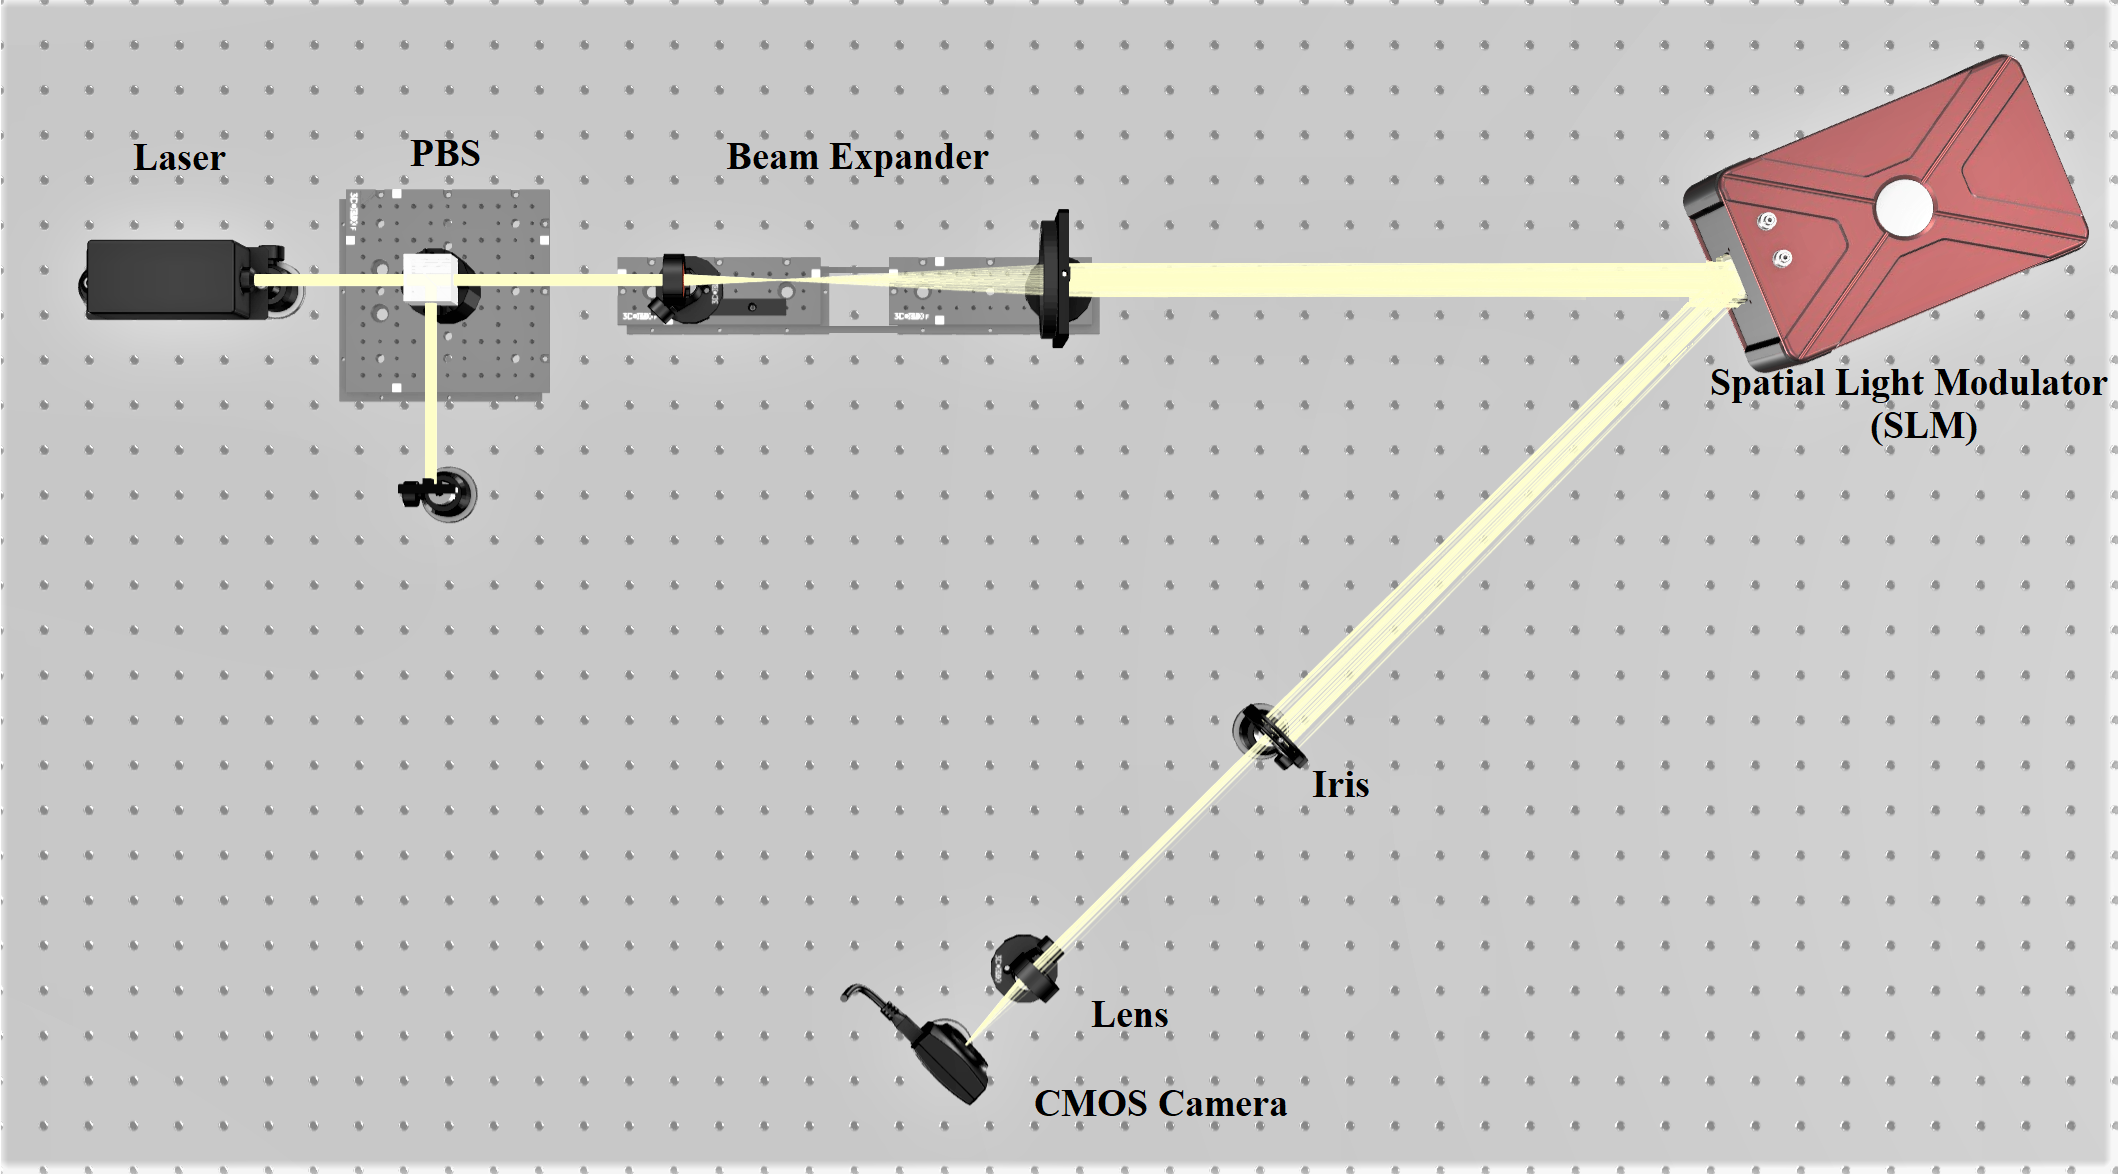
\includegraphics[width=0.8\textwidth]{img/optical_setup.jpg}
\onehalfspacing
\caption{Preliminary Optics setup for the SLM}
\label{fig:optical_setup}
\end{figure}

\begin{figure}[H]
\centering
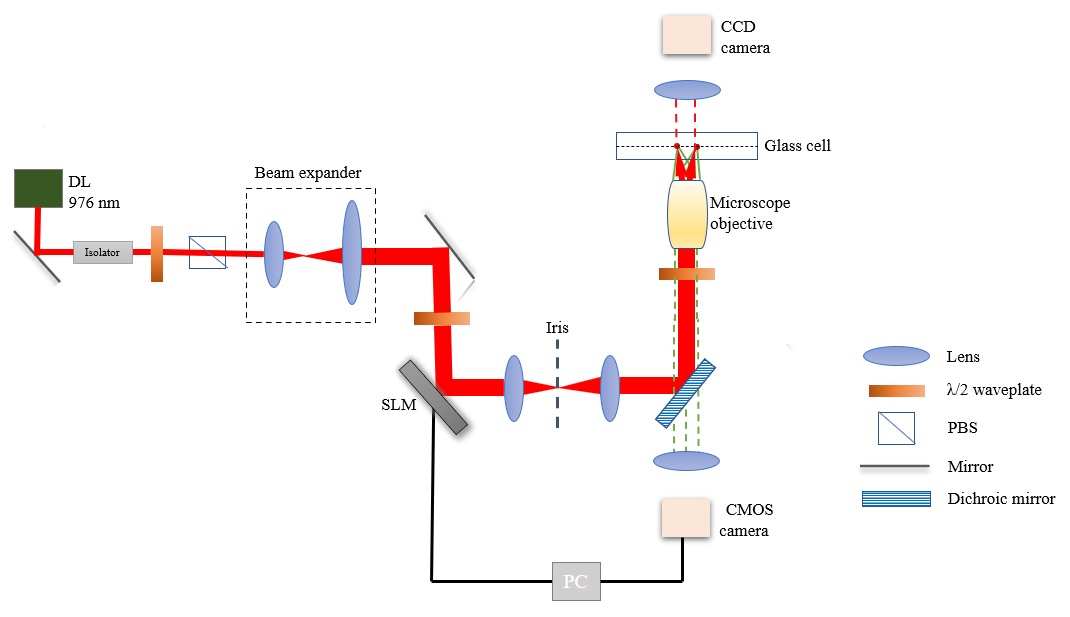
\includegraphics[width=\textwidth]{img/expsetup - Copy.png}
\onehalfspacing
\caption{Proposed Optics setup for trapping atom using optical tweezers}
\label{fig:optical_setup_real}
\end{figure}
\vspace{1em}
\begin{figure}[H]
\centering
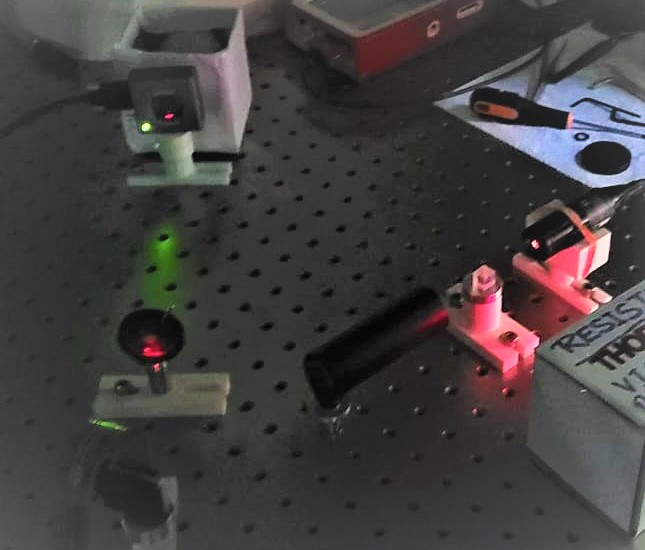
\includegraphics[width=0.75\textwidth]{img/setup on optical table 2.jpeg}
\caption{Optical setup for generating an array of optical tweezers}
\label{fig:optical_setup_lab}
\end{figure}


\subsection{Design of optical tweezers}
From the equation \ref{eq:2} of the previous section, we can see that fourier transform result strongly depends on the $\phi(x,y)$ term. Since we are using phase-only SLM in the experiment. Thus, it becomes crucial to retrieve the phase corresponding to the target intensity distribution of array of optical tweezers.

\subsubsection{Phase-mask generation}
We are using Gerchberg–Saxton(GS) algorithm for the generation phase mask that has to be imprinted on SLM \cite{gerchberg1972practical}. This algorithm was initially used in electron beam microscopy to retrieve phase information from the intensity distribution, which is also known as Error-reduction algorithm \cite{khare2015fourier}. It has now become a usual choice as a phase retrieval algorithm for beam shaping and optical information processing.

The GS algorithm uses the iterative virtual propagation of the light field between the SLM's plane and the lens' focal plane, intending to converge on an appropriate phase to produce a targeted intensity distribution. The algorithm for the GS algorithm is proposed below:

\begin{breakablealgorithm}
\caption{: Gerchberg–Saxton(GS) algorithm}\label{alg:GS}
\algrenewcommand\algorithmicrequire{\textbf{Input:}}
\algrenewcommand\algorithmicensure{\textbf{Output:}}
    \begin{algorithmic}
        \Require  $A_{source}$,  $A_{target}$, $\phi_{r}$, iter
        \Ensure $\phi_{r}$ 
        \State A $\leftarrow$ $exp(i\phi_r)$
        \State $i\leftarrow 0$
        \While{$i<$iter}
            \State $B \leftarrow abs(A_{source})*exp(i*angle(A))$
            \State $C \leftarrow FFT[B]$
            \State $D \leftarrow abs(A_{target})*exp(i*angle(C))$
            \State $A \leftarrow IFFT[D]$
        \EndWhile
        \State $\phi_r \leftarrow angle(A)$
        \State \Return $\phi_r$
\end{algorithmic}
\end{breakablealgorithm}

To determine the adequate phase pattern corresponding to the targeted intensity distribution, we have to numerically implement the above described GS algorithm. For this we have discretized the field in $N_x \times N_y$ matrix in SLM plane with spacing of one cell as $\triangle_x \times \triangle_y$. Thus, we can write discrete complex amplitude in the SLM field as
\begin{eqnarray}
    \label{eq:discrete_A_slm}
    A_{SLM}(m\triangle_x,n\triangle_y) = A_{in}(m \triangle_x, n \triangle_y)e^{i\phi_{mn}},
\end{eqnarray}
\begin{equation}
    A_{SLM}(x,y) = \sum_{m=0}^{N_x-1}\sum_{n=0}^{N_y-1} \delta(x-m \triangle_x) \delta(y-n \triangle_y) A_{in}(m \triangle_x, n \triangle_y)e^{i\phi_{mn}},
\end{equation}
where, $A_{in}(\alpha \triangle_x, \beta \triangle_y)$ is the incident light field on the SLM which is same as the $A_{source}$ described in algorithm \ref{alg:GS} and $\phi_{\alpha \beta}$ is the phase delay obtained using the GS algorithm corresponding to the pixel $\alpha \beta$.
The field in focal plane of the lens is given by \cite{khare2015fourier, nla.cat-vn592477},
\begin{eqnarray}
    \Tilde{A}_f(u \Tilde{\triangle}_x, v \Tilde{\triangle}_x) =  \text{DFT}[A_{SLM}(m\triangle_x,n\triangle_y)],
\end{eqnarray}
\begin{equation}
\label{ref:eq_FocalAmp}
    \Tilde{A}_f(u \Tilde{\triangle}_x, v \Tilde{\triangle}_x) = \sum_{m=0}^{N_x-1}\sum_{n=0}^{N_y-1} A_{in}(m \triangle_x, n \triangle_y)e^{i\phi_{mn}}e^{-2\pi i(mu/N_x + nv/N_y)},
\end{equation}
where, 
\begin{equation}
\label{ref:eq_focaltoslm}
    \Tilde{\triangle}_x=\frac{\lambda f}{L_x}\text{  and  } \Tilde{\triangle}_y=\frac{\lambda f}{L_y}.
\end{equation}
\begin{equation}
\label{ref:eq_slmtofocal}
    \Tilde{L}_x=\frac{\lambda f}{\triangle_x}\text{  and  } \Tilde{L}_y=\frac{\lambda f}{\triangle_y}.
\end{equation}
The equation \ref{ref:eq_FocalAmp} is approximately same as $A_{target}$ and equation \ref{ref:eq_focaltoslm} and \ref{ref:eq_slmtofocal} can be used to estimate the trap distance.







\subsection{Defect free atom array formation}
Let us assume that the probability for atoms getting trapped is 50 percent per site. Therefore, the probability of filling all sites of array with N atoms is $(\frac{1}{2})^N$, which is very small. In order to achieve contiguous arrays of atom with high probability, we have designed our system to capture atoms more than ~2N. Afterwards, we can fill the vacant sites in array from nearby reservoir atoms. Without considering the loss of atom during the transportation for filling vacancies, the probability of filling is now P(N$|$M) given as:
\begin{equation}
    P(N|M) = \Big(\frac{1}{2}\Big)^M \sum_{n=N}^M \binom{M}{n}
\end{equation}
which is greater than $(\frac{1}{2})^N$, where P(N$|$M) is the probability of capturing more than or equal to N atoms out of the starting trap array of M traps \cite{lee2017defect}. 
To accomplish this, we must first determine the arrangement of atoms captured in tweezers, and then identify the voids that must be filled. Following that, we'll undertake path planning for individual atoms to determine their location as a function of time. Then, based on the route, we'll obtain the phase mask and transport the atom.

\subsubsection{Path Planning}
In the suggested approach, atom loss can also occur while the atom is being transported. To minimize the loss, we must complete the transportation in the shortest amount of time and on the shortest available path. This appears to be a combinatorial optimization problem in which we must choose the optimal path from among all feasible paths. The solution to this problem can be found using the Hungarian matching algorithm \cite{lee2017defect}.

\subsubsection*{Hungarian Algorithm}
Finding match for filling the vacancies is a kind of matching problem where we have two sets namely, captured atom configuration $I = \{x_i, y_i\}$ and targeted array $T = \{a_i, b_i\}$ which can be treated as a set of bipartite graph $G(I, T, E)$ where $E$ is each possible edges having cost $c_{ij}$. In the language of graph theory, our problem is to find the best-suited match with the minimum cost (distance between two sites), and matching is guaranteed because of Hall's marriage theorem.

There are several algorithms for solving these sorts of assignment problems, such as the Hopcroft-Karp algorithm and back-propagation (brute force), but the Hungarian Algorithm is considered to be the best since it provides an optimal solution in substantially less time than other algorithms. The Hungarian Technique is a combinatorial optimization algorithm that solves matching problems with a cost restriction. It s known to be efficient as the time complexity of this algorithm is $\mathscr{O}(n^3)$. Hungarian algorithm gives us a matching between two sets $I$ and $T$ of bipartite graph $G(I, T, E)$ minimizing the total cost \cite{golin-notes}. It also guarantee a collision free path because these matching will gives a larger distance to travel than the collision-free matching. Also, in our case we are using cost as $c_{ij} = \{(x_i - a_j)^2 + (y_i - b_j)^2\}$ to avoid the trespassing path \cite{lee2017defect}.\\

The figure 4 depicts the process we have followed to implement movement of atomic tweezers in order to make our array defect-free.

\vspace{1cm}

\begin{figure}[H]
\label{fig:flow chart}
\centering
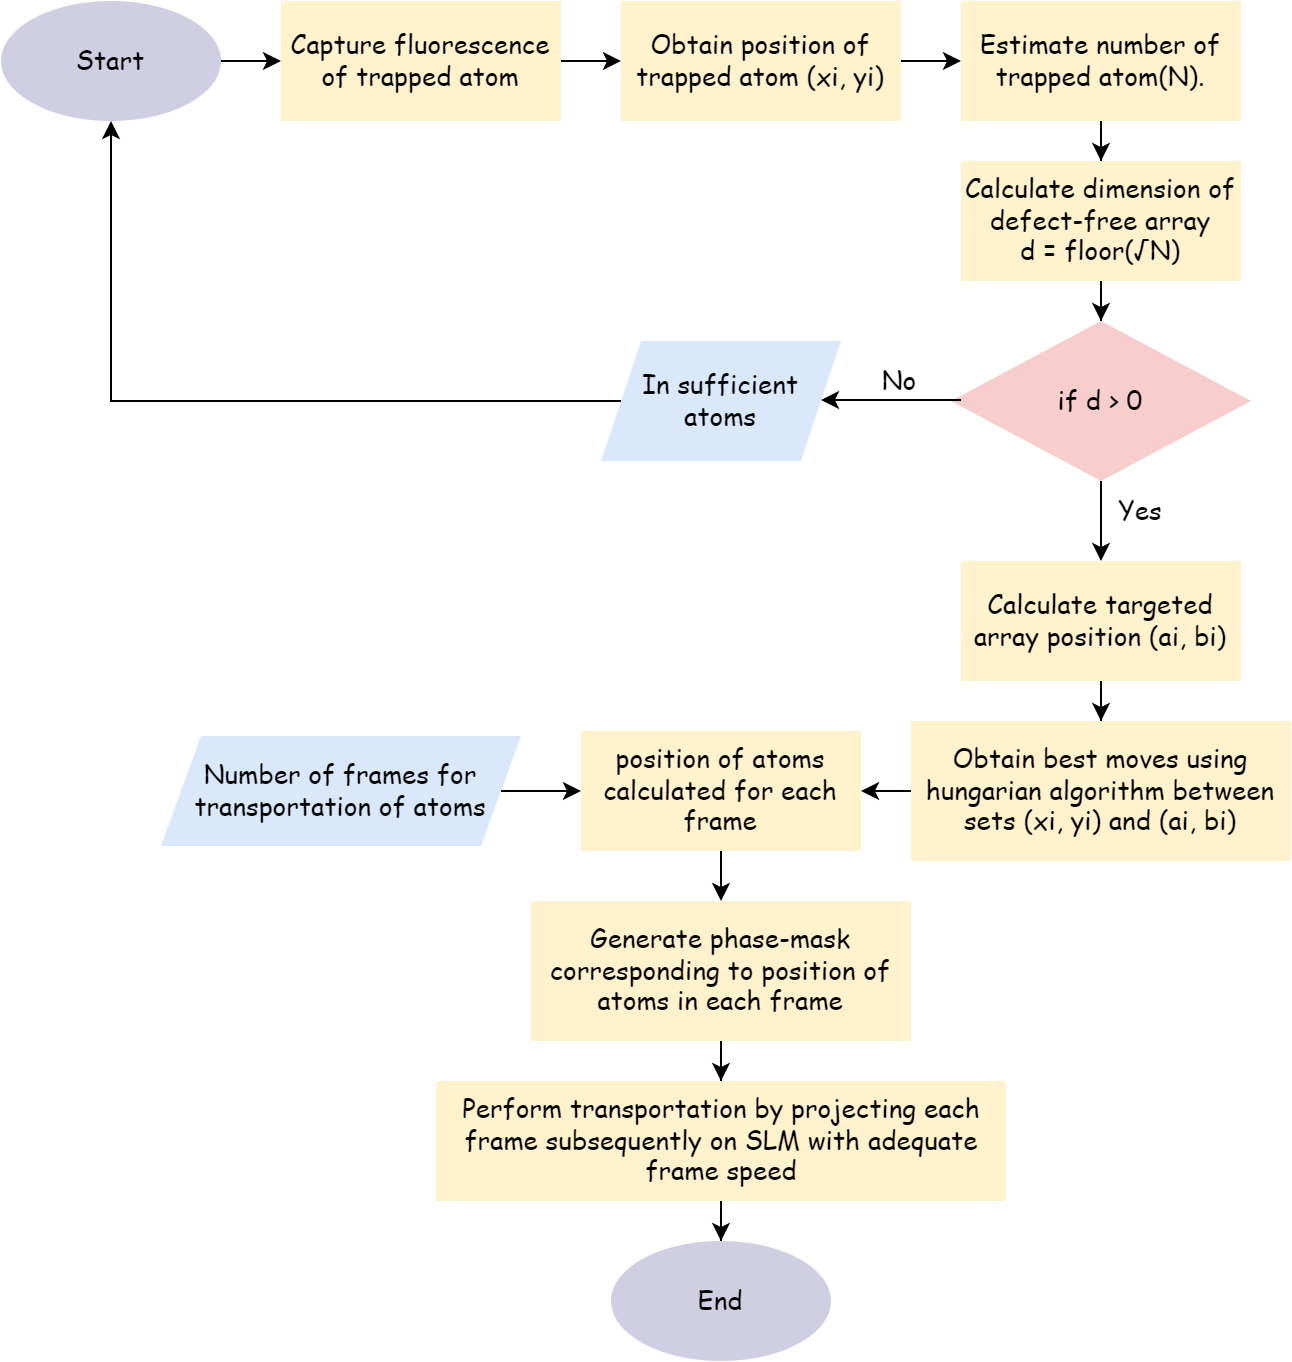
\includegraphics[width=0.9
\textwidth]{img/flowchart.png}
\caption{Flowchart of methods we have followed for the implementation of defect-free atom array}
\end{figure}
